\documentclass[a4paper,10pt]{report}

\def\packagepath{../../../../../preambule}   % path du package princial
\usepackage{\packagepath/preambule}    % utilisation du fichier de configuration

\def\level{BTS }              % Classe
\def\course{CIEL 1}              % Matière
\def\eval{Primitives}

\def\visibleornot{visible}    % visible or invisible
\def\documentpath{./Sources_Latex}
\def\date{C106 - TP2 }
\renewcommand{\arraystretch}{1}  % Ecart dans les tableau

\def\ptsexoA{0}
\def\ptsexoB{0}
\def\ptsexoC{4}
\def\ptsexoD{4}
\def\ptsexoE{1}
\def\ptsexoF{1}
\def\ptsexoG{2}
\def\ptsexoH{1}
\def\ptsexoI{2}
\def\ptsexoJ{2}
\def\ptsexoK{1}

\def\ptstotal{\ptsexoA+\ptsexoB}

\usepackage{hyperref}

\usetikzlibrary{shapes, arrows, positioning}
\usetikzlibrary{shapes.geometric, arrows, positioning, decorations.pathreplacing}

\tikzstyle{etat} = [draw, rounded corners=15pt, minimum width=2.5cm, minimum height=1.2cm, text centered, font=\bfseries]
\tikzstyle{nouveau} = [etat, fill=blue!40]
\tikzstyle{pret} = [etat, fill=green!60]
\tikzstyle{elu} = [etat, fill=yellow!60]
\tikzstyle{bloque} = [etat, fill=red!60]
\tikzstyle{termine} = [etat, fill=white]
\tikzstyle{fleche} = [thick, ->, >=stealth]

\usepackage{float} % Permet d'utiliser [H]
\usepackage[T1]{fontenc}
\begin{document}

%%%%%%%%%%%%%%%%%%%%%%%%%%%%%%%%%%%%%%%%%%%%%%%%%%ù

%\PageGardeSujetBac[Matiere = Numérique et Sciences Informatiques,
%                  Session = 2025,
%                  AffJour=false,
%                  Duree = {3 heures 30},
%                  DernierePage = \pageref{LastPage},
%                  ModeExamen=false
%                  ]
\renewcommand{\labelitemi}{\textbullet} %pour éviter les tirets dans les "itemize" qui apportent confusion avec le signe moins.
%% Début page de garde style BAC

   %%%%%%%%%%%%%%%%%%%%%%%%%%%%%%%%%%%%%%%%%%%%%%%%%%%%%%%%
%\PageGardeSujetBac[clés]

\pagestyle{DS_FP}          % Feuille de style fancy
\NomPrenomNote{}


\exods{\ptsexoA}

\medskip

\begin{easybox*}{Contexte}{}

On modélise le débit d'une connexion internet en Mbps (mégabits par secondes) en fonction de la distance $x$ (en centaines de mètres) par la fonction:

$$f(x)=(ax+b)\e^{-0.5x}$$

$a$ et $b$ sont deux réels à déterminer.
\end{easybox*}

\bigskip

\begin{easybox*}{Conditions expérimentales: }{}


\begin{itemize}
    \item A la sortie du serveur ($x=0$), le débit mesuré est de \textbf{8 Mbps}
    \item la tangente à la courbe représentative de la fonction $f$ à l'origine a  pour coefficient directeur $-2$
\end{itemize}

\end{easybox*}


\medskip

\begin{enumerate}
    \item A l'aide de Géogébra et des conditions expérimentales, déterminer les valeurs des paramètres $a$ et $b$ et donner l'expression de la fonction $f$.
    \begin{answer}{1}{1}  $a= \dotfill$ \hfill $b= \dotfill$ \hfill $f(x)= \dotfill$  \end{answer}
    \item Montrer que la fonction dérivée de $f$ peut s'écrire sous la forme $f'(x)=-(x+2)\e^{-0.5x}$
    \begin{answer}{1}{4}     \end{answer}
    \item Déterminer le signe de la fonction dérivée $f'$ sur $[0; +\infty[$ et compléter le tableau de variation de la fonction $f$ sur $\R$.
    \begin{answer}{1}{9}  
    \begin{minipage}{0.48\linewidth}
        
    \end{minipage}\hfill
    \begin{minipage}{0.48\linewidth}
        
    \begin{center}
    \begin{tikzpicture}
    \tkzTabInit[lgt=2,espcl=3.5]
    {$x$ / 1, $signe \, f'(x)$ / 1, $var \, f$ / 1}
    {$0$, $+\infty$}
    \tkzTabLine{}
    \tkzTabVar{}
    \end{tikzpicture}
\end{center}
    \end{minipage}
    
   \end{answer}

   \pagebreak
   \thispagestyle{DS_LP}
    \item Déterminer l'équation de la tangente à la courbe représentative de la fonction $f$ au point d'abscisse 0.
        \begin{answer}{1}{4}     \end{answer}

    \item On considère que le débit de la connexion internet est considéré comme non acceptable si il est inférieur ou égal à 2 Mbps. Déterminer à partir de quelle distance le débit n'est plus acceptable et qu'il faudra alors envisager d'installer un répéteur. On arrondira cette distance au mètre près.

    \begin{answer}{1}{1}     \end{answer}

\end{enumerate}

\exods{\ptsexoB}

\medskip

\begin{easybox*}{Reconstitution du volume de données transféré}{}

On s'intéresse au volume total de données transféré sur une période donnée. On modèle le débit instantané (en Mbps) à l'instant $t$ (en minutes) par:
$$p(t)=3t\e^{-0.5t}$$

\end{easybox*}

Un ingénieur propose que la fonction $G(t) = (-6t - 12)\e^{-0.5t}$ représente le volume total de données transféré (en Mo) depuis le début de la transmission jusqu'à l'instant $t$.

\medskip


\begin{enumerate}
    \item Vérifier que $G$ est une primitive de la fonction $p$.
        \begin{answer}{1}{5}     \end{answer}
\item La transmission commence sans données transférées. Déterminer alors la primitive $H$ de la fonction $p$ vérifiant $H(0)=0$.
    \begin{answer}{1}{3}     \end{answer}
    \item Déterminer le volume total de données transféré au bout de 10 minutes, arrondir à l'unité près.
        \begin{answer}{1}{1}     \end{answer}

\end{enumerate}
\end{document}


        \begin{answer}{1}{1.5} 

            $f'(x)=$
\end{answer}

    \begin{minipage}{0.28\linewidth}
    \item Déterminer par le calcul le signe de la fonction dérivée sur $\R$.
\end{minipage}\hfill
\begin{minipage}{0.68\linewidth}
        \begin{answer}{1}{4} 

            
\end{answer}
\end{minipage}

\begin{minipage}{0.28\linewidth}
    \item Compléter alors le tableau de variation de la fonction $f$ sur $\R$..
\end{minipage}\hfill
\begin{minipage}{0.68\linewidth}
        \begin{answer}{1}{3.6} 

            
\end{answer}
\end{minipage}

\begin{minipage}{0.28\linewidth}
    \item Déterminer par le calcul l'équation de la tangente à la courbe représentative de la fonction $f$ au point d'abscisse 0.
\end{minipage}\hfill
\begin{minipage}{0.68\linewidth}
        \begin{answer}{1}{3.5} 

            
\end{answer}
\end{minipage}


\end{enumerate}

\pagebreak
\thispagestyle{DS_LP}

\exods{\ptsexoC}

On considère la fonction $f$ définie sur $\R$ par $f(x)=(ax-2)\e^{-bx}$ où $a$ et $b$ sont deux réels à déterminer. On note $\mathcal{C}_f$ la courbe rerpésentative de la fonction $f$ dans un repère orthonormé.


On souhaite que $a$ et $b$ vérifient les conditions suivantes:
\begin{itemize}
    \item La courbe passe par le point $A(-0,5; 0)$.
    \item La tangente à la courbe $\mathcal{C}_f$ au point d'abiscisse 0 est égal à 2.
\end{itemize}

\begin{enumerate}

\begin{minipage}{0.48\linewidth}
        \item Déterminer grace à Géogebra les réels $a$ et $b$ vérifiant ces conditions.
\end{minipage}\hfill
\begin{minipage}{0.48\linewidth}
        \begin{answer}{1}{1} 

            $a= \dotfill$ \hfill $b= \dotfill$
\end{answer}
\end{minipage}

\begin{minipage}{0.3\linewidth}
        \item Déterminer par le calcul l'équation de la tangente à la courbe $\mathcal{C}_f$ au point d'abiscisse 0.


\end{minipage}\hfill
\begin{minipage}{0.69\linewidth}
        \begin{answer}{1}{3} 

            
\end{answer}
\end{minipage}
    
    
\begin{minipage}{0.28\linewidth}
    \item Compléter alors le tableau de variation de la fonction $f$ sur $\R$..
\end{minipage}\hfill
\begin{minipage}{0.68\linewidth}
        \begin{answer}{1}{3.6} 
\begin{center}
    \begin{tikzpicture}
    \tkzTabInit[lgt=2,espcl=6.5]
    {$x$ / 1, $f'(x)$ / 1, $f(x)$ / 1}
    {$-\infty$, $+\infty$}
    \tkzTabLine{}
    \tkzTabVar{}
    \end{tikzpicture}
\end{center}
            
\end{answer}
\end{minipage}
\end{enumerate}


\exods{\ptsexoD}


Soit $f$ la fonction définie sur $]0; \, +\infty[$ par $f(x)=a\ln(x)+x^2$ où $a$ est un réel à déterminer.

On souhaite que $a$ soit tel que le nombre dérivé de la fonction $f$ en 1 soit égal à 0.

\begin{enumerate}
\begin{minipage}{0.48\linewidth}
        \item Déterminer grace à Geogebra le réel $a$  vérifiant cette condition.
\end{minipage}\hfill
\begin{minipage}{0.48\linewidth}
        \begin{answer}{1}{1} 

            $a= \dotfill$ 
\end{answer}
\end{minipage}


        \item Déterminer l'expression de la fonction dérivée de $f$ et étudier son signe.
        \begin{answer}{1}{7}\end{answer}

        \begin{minipage}{0.28\linewidth}
    \item Compléter alors le tableau de variation de la fonction $f$ sur $\R$..
\end{minipage}\hfill
\begin{minipage}{0.68\linewidth}
        \begin{answer}{1}{3.6} 
\begin{center}
    \begin{tikzpicture}
    \tkzTabInit[lgt=2,espcl=6.5]
    {$x$ / 1, $f'(x)$ / 1, $f(x)$ / 1}
    {$0$, $+\infty$}
    \tkzTabLine{}
    \tkzTabVar{}
    \end{tikzpicture}
\end{center}
            
\end{answer}
\end{minipage}

\end{enumerate}




\end{document}








